\documentclass[]{article}
\usepackage{graphicx}
\usepackage{float}
\usepackage[english]{babel}
\usepackage{titlepic}
\usepackage{hyperref}
\usepackage{float}
\usepackage{multirow}
\usepackage{floatflt}
\usepackage[style=authoryear-ibid,backend=bibtex]{biblatex}
\hypersetup{
	citecolor=black,
	urlbordercolor={1 1 1},
	colorlinks=true,
	linkcolor=blue,
	filecolor=blue,      
	urlcolor=blue,
}
\addbibresource{sample.bib}
%Load 
\begin{document}
	\begin{titlepage}
		\centering
		\title{UI design for mobile systems
		}
		\author{by Christoffer Lundström}
		\date{\centering
			July 7, 2019\endgraf\vspace{2cm}\endgraf
			Development of Mobile Applications - 5DV209\endgraf
			Examinator: Johan Eliasson\endgraf
			}
	
		\titlepic{
\includegraphics[width = 40mm]{logo.png}}	
		\maketitle
		\thispagestyle{empty}
	\end{titlepage}
	\newpage
	\tableofcontents
	\thispagestyle{empty}
	\newpage
	
\begin{flushleft}
\section{Introduction}

This report will cover the structural design of a prototype port for Windows Calendar on PC to Android by abstracting and analysing the UI elements and functionalities of the application and converting these to appropriate entities according to the \textit{MVC-pattern}. It will cover basic requirements of the application such as placement and design of Views, description of controllers and models.\medskip


The prototype will follow UI guidelines of Androids \textit{\href{https://material.io/design/}{Material design}} and general design- principles.
Furthermore a comparison will be made between \textit{Material Design} and \textit{\href{https://developer.apple.com/design/human-interface-guidelines/ios/overview/themes/}{iOS human interface guidelines}} to show how an adaptation of the prototype could be produced for iOS.

\subsection{Purpose}

By examining an existing application and applying design principles for Android and iOS we will gain a practical understanding of user interface design for mobile applications, which in extension is a requirement for the course\medskip.

Another purpose of this assignment is to prioritize functionalities and reflect upon the importance and usefulness of each interaction as there generally is a limited amount of screen space in a mobile environment.

\newpage
\section{Procedure \& materials}

Windows 10 PRO and the embedded Windows Calendar(fig 1) version 16005 is used in this experiment.\newline
The main method of analysing the Calendar application in this assignment is by visually and practically examining its use cases and determining the most suitable view or controller in an Android setting.

\begin{figure}[H]
	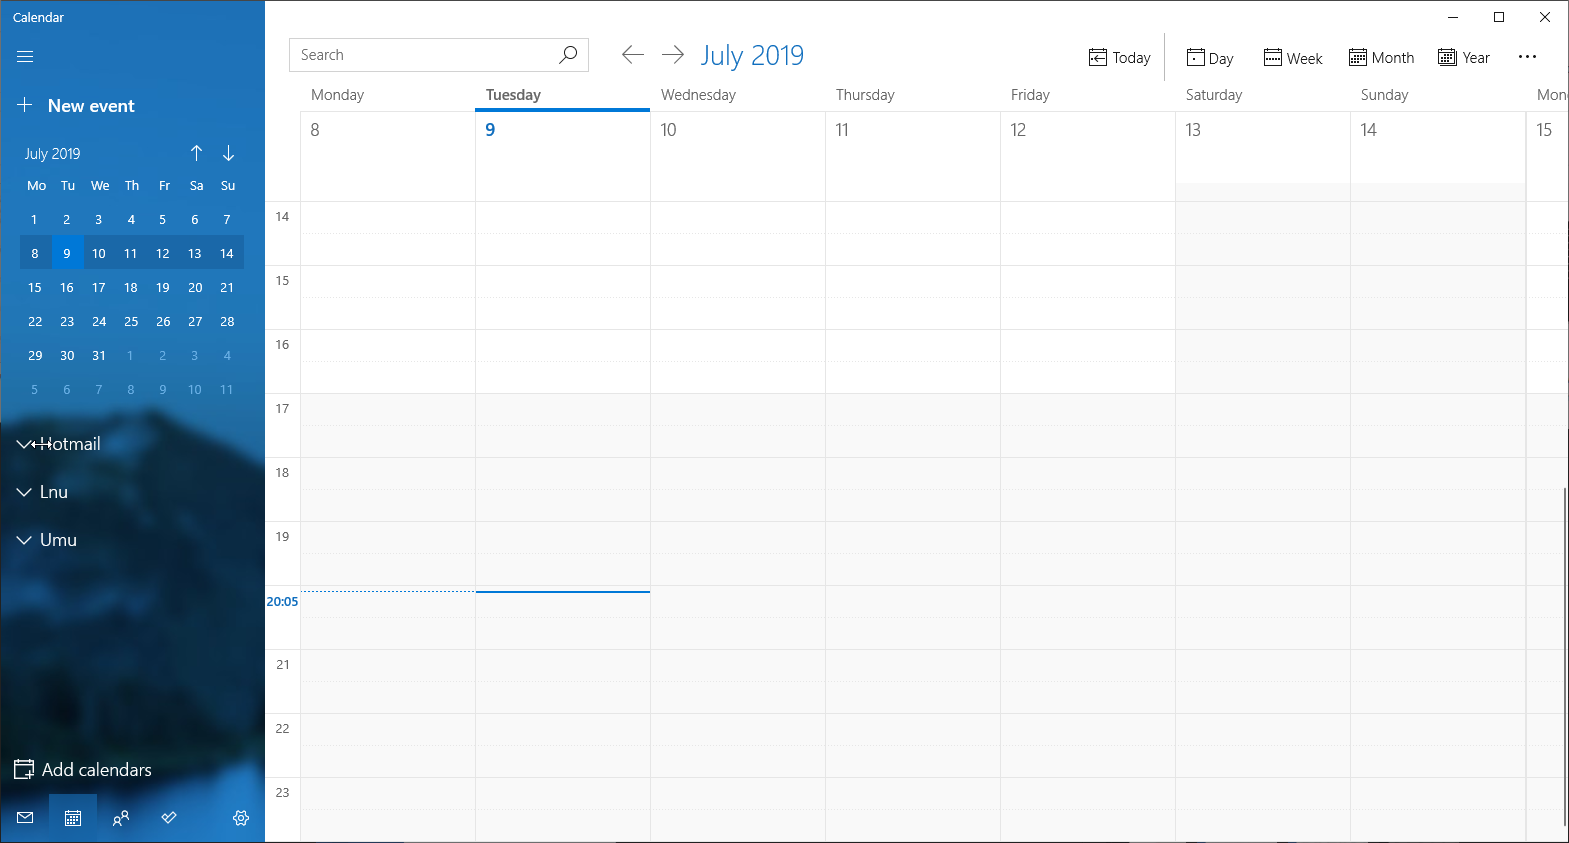
\includegraphics[width=\linewidth, height=60mm]{weekview.png}
	\caption{Week and month UI of Windows calendar.}
	\label{fig:week_view}
\end{figure}

By breaking down each component and use case the conversion to Android will be significantly easier to comprehend.\medskip

Android Studio v.3.4.1 by JetBrains is used to produce some of the interface designs.

Photoshop CC 2017 is used for an overview design and initial design template.


\newpage
\section{Results}
\subsection{Requirements Analysis}


\subsubsection{Functional}
This section will break down individual buttons and components to a few of the most important Use Cases required by the prototype.\medskip

\begin{center}
\noindent\fbox{%
	\parbox{10cm}{%
		\begin{center}
			Use-Case - View events
		\end{center}
		
		Pre-condition: None.\newline
		Post-condition: None.\newline
		
		Main Scenario:\newline
		1. User wants to view events on a particular date.\newline
		2. User selects a date.\newline
		3. User is presented with a view of detailed information of events.\newline
	}
}\medskip



\noindent\fbox{%
	\parbox{10cm}{%
		\begin{center}
			Use-Case - Add events
		\end{center}
		
		Pre-condition: None.\newline
		Post-condition: User is returned to Calendar-View.\newline
		
		Main Scenario:\newline
		1. User wants to add an event.\newline
		2. User presses Add button.\newline
		3. User is presented with an empty dialog form.\newline
		4. User enters Name, Location, Date, Time and Description of event.\newline
		5. User saves event.\newline
		
		Alternative Scenario: \newline
		5. User presses Back or Cancel.\newline
	}
}\medskip

\noindent\fbox{%
	\parbox{10cm}{%
		\begin{center}
			Use-Case - Modify event
		\end{center}
		
		Pre-condition: User has selected a date with existing events.\newline
		Post-condition: User is returned to Calendar-view.\newline
		
		Main Scenario:\newline
		1. User wants to modify event.\newline
		2. User presses event in detail view.\newline
		3. Dialog view is presented with details of event.\newline
		4. User modifies details.\newline
		5. User presses save.\newline
		
		Alternative Scenario:\newline
		5. User presses back or cancel.\newline
	}
}\medskip

\noindent\fbox{%
	\parbox{10cm}{%
		\begin{center}
			Use-Case - Delete event
		\end{center}
		
		Pre-condition: User has selected a date with existing events.\newline
		Post-condition: None.\newline
		
		Main Scenario: \newline
		1. User wants to delete event.\newline
		2. User right-swipes or long-presses event item.\newline
		3. User is presented with confirmation dialog.\newline
		4. User confirms action.\newline
		
		Alternative Scenario: \newline
		4. User aborts confirmation.\newline
	}
}\medskip
\end{center}


The windows calendar consists of four overviews. Year, month, week and day. The yearly overview will be intentionally left out of the prototype due to the fact that display of dates would have to be less than 10sp which is non compliant to material design and unviable for a small screen\parencite{typog}.\medskip

\subsubsection{Non functional}
This section will cover requirements related to performance, accessibility, modifiability and scalability.\medskip

To make sure the Calendar runs smoothly one important aspect of the design is to load events dynamically based on the date. This means not loading the entire event-database into memory but rather run queries against a database or local file. It wouldn't make sense to load passed events unless specifically asked for. A better approach would be to load the currently viewed month's events. This will not only make the application faster, but also make it more maintainable and scaleable.\medskip

Another requirement of our prototype is to keep the user interface clear, robust and specific.
Meaning having a clear UI with sufficient contrast ratios and structure to nudge the user through the application. It should be clear what is asked from the user \parencite{acc}.
\medskip

Modifiability of the calendar will be handled programmatically by keeping elements subdivided into fragments and adhering to an \textit{MVC} pattern. This will ensure loose coupling of the application.

\subsection{Design}

\subsubsection{Overview}

\begin{figure}[H]
	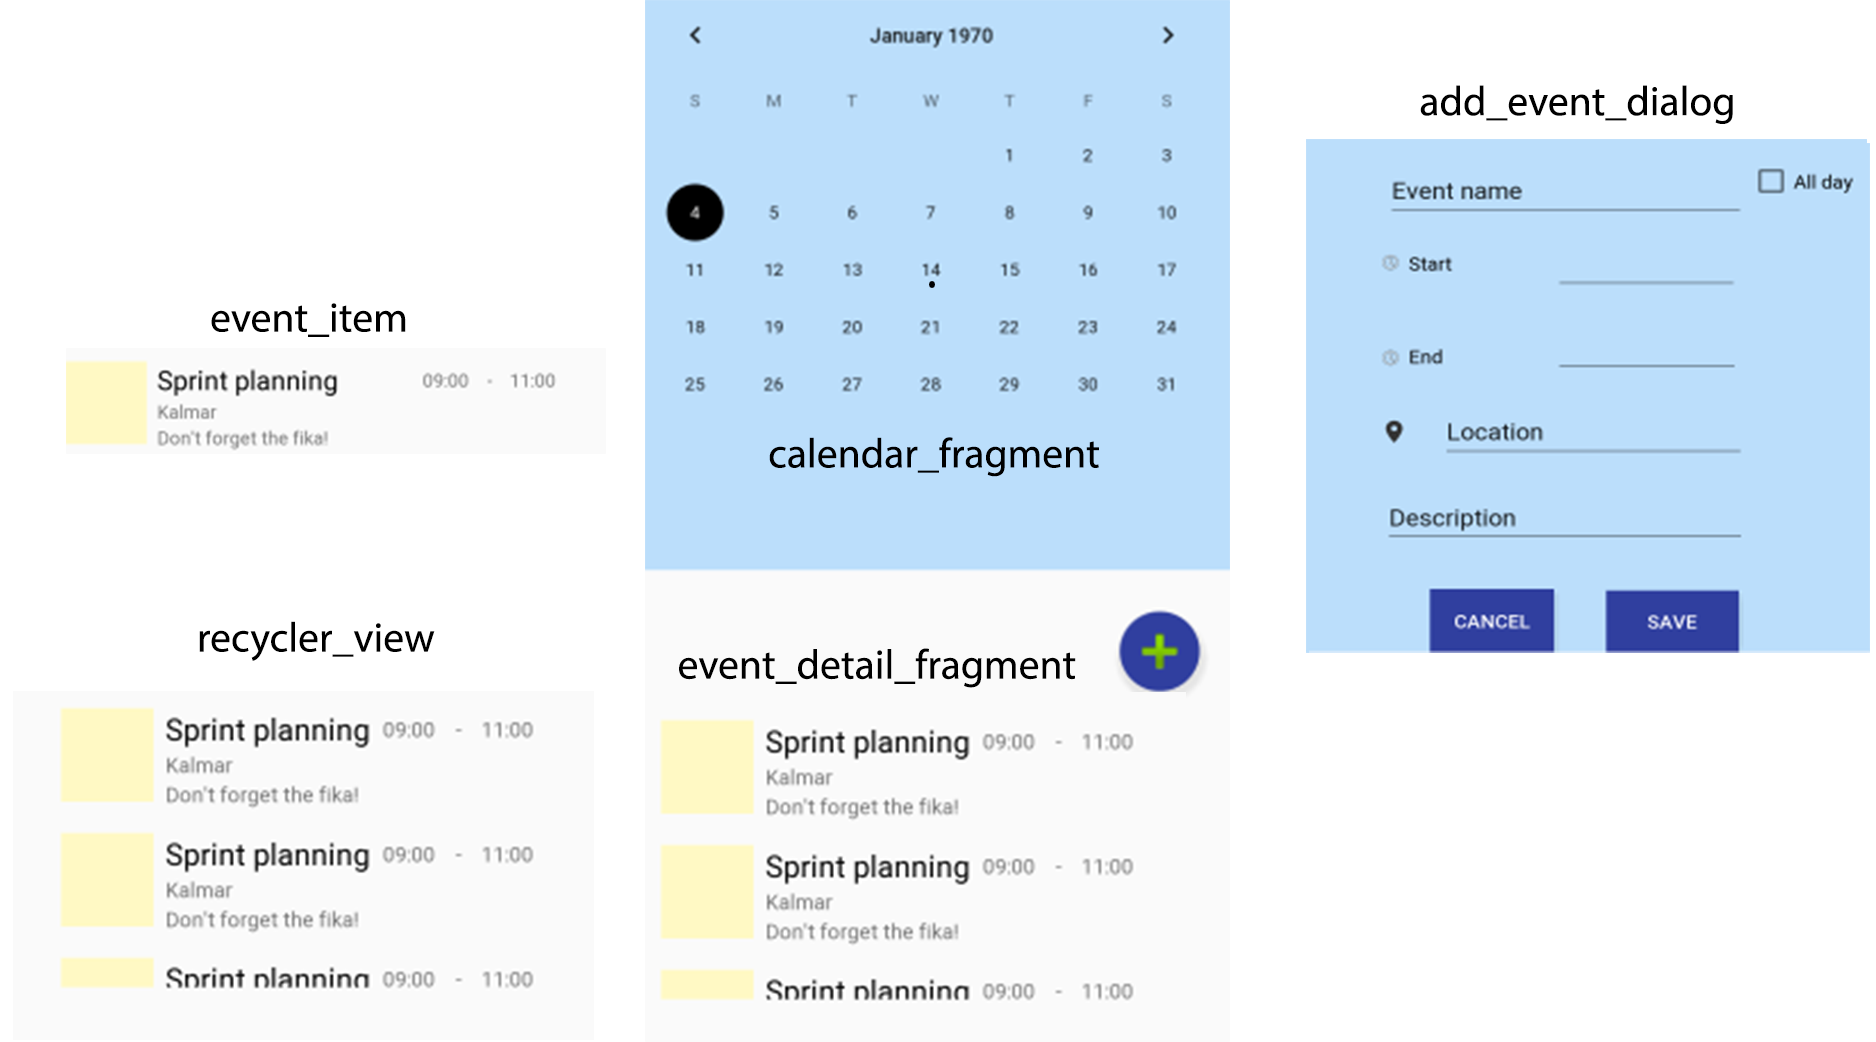
\includegraphics[width=\linewidth, height=60mm]{img/design.png}
	\caption{The different parts that make up the main calendar view.}
	\label{fig:design}
\end{figure}

\begin{figure}[H]
	\centering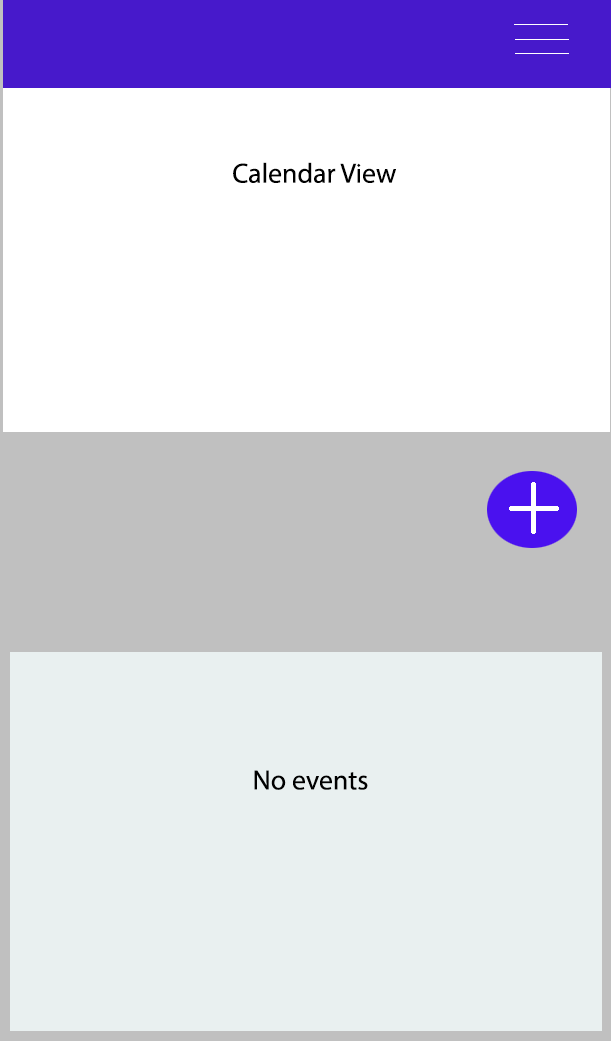
\includegraphics[scale=0.13]{img/initial_design.png}
	\caption{Initial design template.}
	\label{fig:initial_design}
\end{figure}



\newpage

\subsubsection{Calendar}

\begin{floatingfigure}[r]{0.3\linewidth}
	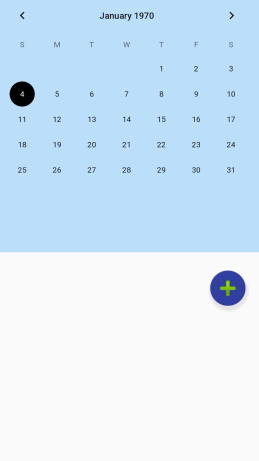
\includegraphics[scale=0.7]{img/date_fragment.png}
	\caption{The first fragment includes the calendar and a button.}
	\label{fig:calendar}
	\vspace{\dimexpr0.3\baselineskip-\topskip}
\end{floatingfigure}

The main activity will be empty except for a single fragment container.
It will be the main controller and hold a fragment-manager which is responsible for initializing the first calendar fragment.\medskip

The calendar fragment will be responsible for date-selection and return a Date object to the main activity which in turn creates the event detail fragment and passes the data via a bundle. In general all data-transactions between fragments are done via the hosting activity \parencite{dev:1}.\medskip

The calendar is placed at the top of our focus hierarchy with a high contrast material background as this should be the first point of focus for the user \parencite{button:2}.\smallskip


Following the calendar a green \textit{Add event} button is placed within an easily reached  region of the screen, both for one-hand and two-hand users. The button has a touch area of 48dp and is coloured in a stark contrast with a slight shadow and elevation to emphasize its presence. Furthermore the button is placed just above the event detail area to make the purpose clear \parencite{button:1}.


\begin{figure}[H]
	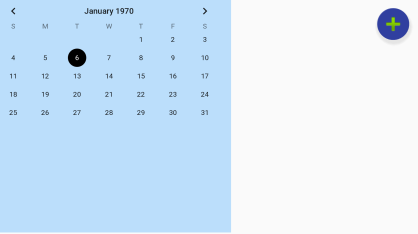
\includegraphics[scale=0.7]{img/landscape.png}
	\caption{Landscape view.}
	\label{fig:design_landscape}
\end{figure}


\newpage


\left\subsubsection{Event details}
%\left funkar bra



\begin{floatingfigure}[r]{0.3\linewidth}
	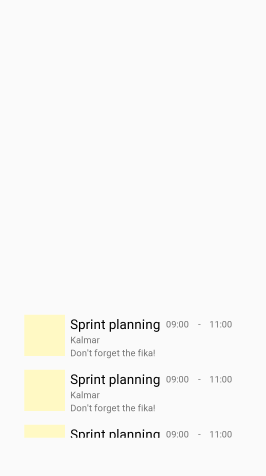
\includegraphics[scale=0.7]{img/recycler_view.png}
	\caption{Event detail fragment with a Recycler view.}
	\label{fig:recycler_view}
	\vspace{\dimexpr0.3\baselineskip-\topskip}
\end{floatingfigure}

The next part of our prototype is the event detail fragment which will provide information regarding the specified time, location and description of the events on the selected date.\medskip

Each event is marked with a colour to clearly separate its regions \parencite{text}.
\newline The fragment fills the rest of the screen\newline with a scrollable list of event items. This fragment will handle an internal recycler view responsible for rendering the event item model data. Before rendering a view the fragment controller should retrieve relevant data by querying a local or external database with the date passed to the fragment with the bundle.\medskip

\begin{figure}[H]
	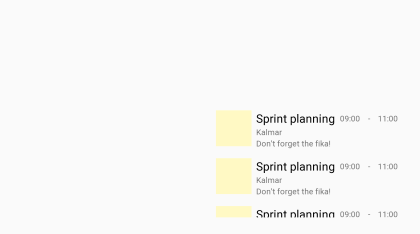
\includegraphics[scale=0.7]{img/recycler_landscape.png}
	\caption{Recycler landscape view.}
	\label{fig:design_landscape}
\end{figure}

\newpage

\left\subsubsection{Add event dialog}

\begin{floatingfigure}[r]{0.4\linewidth}
	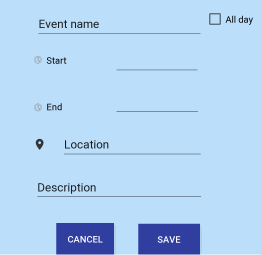
\includegraphics[scale=0.7]{img/dialog.png}
	\caption{The add event view.}
	\label{fig:dialog}
	\vspace{\dimexpr0.3\baselineskip-\topskip}
\end{floatingfigure}

This dialog is controlled by the Calendar fragment. By adding a click-listener to the \textit{add event} button a new instance of the dialog will be created by the main activity fragment-manager.\medskip

The fields of this view are based on a custom event item model which is later used for storing events. It is important that this model implements a way to serialize or parse data between fragments, servers and storage locations \parencite{parcel}.\medskip

Design of this dialog is simplistic but expresses its intent clearly with icons\\ recommended in material design \parencite{icons:1}. It also follows the blue material theme as its parent fragment \parencite{button:1}.


\left\subsubsection{iOS adaptation}

To adapt our prototype to iOS there are some changes and additions which could be made.
First of all is to have a clear hierarchical navigation. The current prototype supports this as it basically contains two different views; calendar and the event view modal/dialog. Our dialog is dismissed by navigating using back. Another way to dismiss the dialog could be to use a swiping motion \parencite{modality}.
Furthermore the dialog should be converted to a \textit{popover}. This makes the focus point clear as the background is dimmed \parencite{popover}.
\medskip

When a new event has been added or an existing has been modified a feedback notification could be added at the bottom of the screen similar to a \textit{toast} in Android\parencite{feedback}.\medskip

Animation is also a big part of interfacing with a user and thus a slider which fills the event detail row could be added for additional clarity when pressing down on a event. This could be an indication for modifying or deleting the event \parencite{animation}.\medskip

Additionally a two-color system for the current theme could be added to represent a dark and light mode \parencite{color}.\medskip

Like \textit{material design} the \cite{elevation} uses elevation of elements to separate content from backgrounds or foregrounds. This is already present in our prototype and doesn't need further adaptation.

As user feedback and immediate response is an important aspect of HIG a loading bar or indicator could be added when the event detail fragment queries the database for event content asynchronously \parencite{progress}.


\left\section{Discussion}

Material design and iOS human interface are two very similar principles of design which overlap in many areas such as content elevation, touch controls and especially navigation. Other differences are more subtle such as dimming of foreground with popovers or navigating with tabs. Because both of these guidelines have a friendly user-experience as the end goal and follow similar design patterns prototyping is easier, especially for tiny projects like this one. I suspect that the differences become more apparent and substantial as projects scale in size, perhaps there are more limiting factors to UI designs from a technical perspective when comparing activities, fragments etc. to the iOS framework.\medskip

This design may seem trivial compared to the fully fledged Windows calendar but the key functionalities of the calender are covered and designed with the mobile user in mind. As mentioned in \cite{joshclark:1} by Josh Clark:

\begin{quote}
"The point is not to arbitrarily strip out features and content, but a matter more of organizing and prioritizing."
\end{quote}

To summarize I think that this project has been quite insightful as to current methods of UI development and I look forward to pursuing these schools of design further.
\newpage


\left\section{References}
\printbibliography[title={Online sources}]

\end{flushleft}
\end{document}          
